% ==================================================================
% Safety loss + anchor loss + best marginal result.
% FRAMES ONLY -- \input this into main.tex (preamble lives there).
%
% Assumes the preamble already loads: beamer, amsmath, amssymb,
% booktabs, xcolor, tikz.  The guarded block below adds the tikz
% library, colors, and \good/\bad/\carbox ONLY if missing, so it is
% safe to keep even when your preamble already defines them.
% ==================================================================
\usetikzlibrary{arrows.meta}

% ---- colors (namespaced so they don't clobber yours) -------------
\definecolor{safetyC}{HTML}{CE4325}
\definecolor{anchorC}{HTML}{0C8571}
\definecolor{policyC}{HTML}{37699F}
\definecolor{edgeC}{HTML}{2A303A}
\definecolor{driveC}{HTML}{E4E8EE}
\definecolor{safetySoft}{HTML}{F6DBD2}
\definecolor{anchorSoft}{HTML}{CDE8E1}
\definecolor{policySoft}{HTML}{D8E3F0}

% ---- emphasis macros (fallbacks; your preamble's win) ------------
\providecommand{\good}[1]{\textcolor{anchorC}{#1}}
\providecommand{\bad}[1]{\textcolor{safetyC}{#1}}

% ---- a rotated ego bounding box: {cx}{cy}{angle}{fill}{draw} ------
\providecommand{\carbox}[5]{%
  \draw[fill=#4,draw=#5,line width=0.9pt,rounded corners=1.5pt,
        rotate around={#3:(#1,#2)}]
    (#1-0.55,#2-0.3) rectangle (#1+0.55,#2+0.3);}


% ##################################################################
\section{Safety loss}
% ##################################################################

% ------------------------------------------------------------------
\begin{frame}{Safety loss: the clearance the indicator throws away}
  \small
  \begin{columns}[T]
    \column{0.52\textwidth}
    Waymax scores geometry only as \textbf{indicators} --- \texttt{offroad},
    \texttt{overlap} are $0/1$, zero gradient everywhere. We recover the
    \emph{continuous clearance} they threshold. Two quantities, metres,
    positive $=$ safe, whose sign \emph{is} the metric's boundary:
    \[
      \min_{k}\, c^{\text{edge}}_{k} < 0 \;\Leftrightarrow\; \texttt{offroad}=1,
      \qquad
      c^{\text{ag}}_{j} < 0 \;\Leftrightarrow\; \texttt{overlap}=1 .
    \]
    One-sided barrier: flat when clear, knee of width $\tau$ at the margin,
    unbounded ramp inside (gradient saturates at the weight, does not vanish):
    \[
      \mathrm{barrier}(c) \;=\; \tau\,\operatorname{softplus}\!\Big(\tfrac{m-c}{\tau}\Big).
    \]
    Applied \textbf{per corner} and \textbf{per agent} and \textbf{summed} ---
    two corners near the edge cost more than one:
    \[
      \mathcal{L}_{\text{safety}}=\!\sum_{t\in W}\!\Big[
        \sum_{k=1}^{4}\!\mathrm{barrier}(c^{\text{edge}}_{k};m_e,\tau_e)
        +\!\!\sum_{j\in\text{ag}}\!\!\mathrm{barrier}(c^{\text{ag}}_{j};m_a,\tau_a)
      \Big].
    \]
    \footnotesize Margins from the expert's p01 clearance:
    edge $m{=}0.30,\tau{=}0.15$; agent $m{=}0.75,\tau{=}0.25$.

    \column{0.48\textwidth}
    \centering
    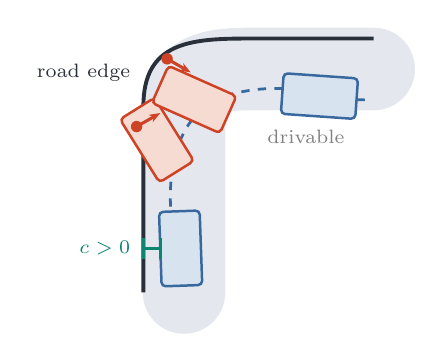
\begin{tikzpicture}[scale=0.86,>={Stealth[length=4pt]},font=\scriptsize]
      % drivable band (thick light stroke) + inner road edge
      \draw[driveC,line width=1.05cm,line cap=round,line join=round]
        (2.6,0.3) -- (2.6,3.0) .. controls (2.6,3.55) and (3.05,3.6) .. (3.6,3.6) -- (5.4,3.6);
      \draw[edgeC,line width=1.4pt]
        (2.0,0.3) -- (2.0,3.05) .. controls (2.0,4.0) and (2.7,4.05) .. (3.55,4.05) -- (5.4,4.05);
      \node[edgeC,anchor=east] at (1.95,3.55) {road edge};
      \node[gray] at (4.4,2.6) {drivable};
      % ego trajectory (policy, dashed)
      \draw[policyC,dashed,line width=1pt]
        (2.55,0.6) .. controls (2.15,2.2) and (2.6,3.0) .. (3.2,3.2)
                   .. controls (4.2,3.5) and (4.8,3.1) .. (5.3,3.15);
      % safe entry box (+ clearance)
      \carbox{2.55}{0.95}{-88}{policySoft}{policyC}
      \draw[anchorC,line width=1pt] (2.25,0.95) -- (2.0,0.95);
      \draw[anchorC,line width=1pt] (2.25,0.8)--(2.25,1.1);
      \draw[anchorC,line width=1pt] (2.0,0.8)--(2.0,1.1);
      \node[anchorC,anchor=east] at (1.95,0.95) {$c>0$};
      % two violating boxes (cutting the corner)
      \carbox{2.2}{2.55}{-58}{safetySoft}{safetyC}
      \carbox{2.75}{3.15}{-24}{safetySoft}{safetyC}
      % exit box, safe
      \carbox{4.6}{3.2}{-4}{policySoft}{policyC}
      % corner violations: dot + outward gradient push
      \fill[safetyC] (1.9,2.75) circle (2.4pt);
      \draw[safetyC,line width=1.1pt,->] (1.9,2.75) -- (2.25,2.95);
      \fill[safetyC] (2.35,3.75) circle (2.4pt);
      \draw[safetyC,line width=1.1pt,->] (2.35,3.75) -- (2.7,3.55);
    \end{tikzpicture}\\[2pt]
    {\scriptsize\textcolor{safetyC}{$\bullet$}~corner in violation
     ~~\textcolor{policyC}{--\,--}~ego path}
  \end{columns}
  \vspace{2pt}
  \footnotesize The barrier's zero level set \emph{is} \texttt{is\_offroad}'s
  decision boundary --- trustworthy by construction, not approximation.
\end{frame}

% ------------------------------------------------------------------
\begin{frame}{Where the safety loss enters: two narrow windows}
  \small
  Evaluated on the \textbf{finished} candidate ($t{=}0$), over the states the
  policy actually reaches --- but it only \emph{enters} through two windows.
  \begin{columns}[T]
    \column{0.5\textwidth}
    \begin{block}{1 -- last $k{=}10$ reverse steps}
    \centering
    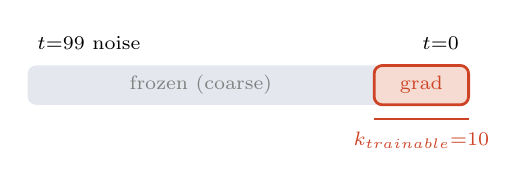
\begin{tikzpicture}[font=\scriptsize]
      \fill[driveC,rounded corners=3pt] (0,0) rectangle (5.6,0.5);
      \fill[safetySoft,rounded corners=3pt,draw=safetyC,line width=1pt] (4.4,0) rectangle (5.6,0.5);
      \node[anchor=west] at (0,0.78) {$t{=}99$ noise};
      \node[anchor=east] at (5.6,0.78) {$t{=}0$};
      \node[gray] at (2.2,0.25) {frozen (coarse)};
      \node[safetyC] at (5.0,0.25) {grad};
      \draw[safetyC,line width=1pt] (4.4,-0.18)--(5.6,-0.18);
      \node[safetyC,anchor=north] at (5.0,-0.22) {$k_{\text{trainable}}{=}10$};
    \end{tikzpicture}\\[3pt]
    {\scriptsize residual xy noise: $t9{\to}16.7$m, $t2{\to}5.8$, $t0{\to}2.5$.}
    \end{block}
    Low-noise end sets the \emph{precise geometry} of the turn; high-noise steps
    pick the coarse manoeuvre and stay frozen.

    \column{0.5\textwidth}
    \begin{block}{2 -- the executed window}
    \centering
    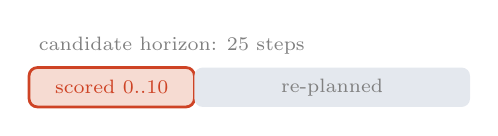
\begin{tikzpicture}[font=\scriptsize]
      \fill[safetySoft,rounded corners=3pt,draw=safetyC,line width=1pt] (0,0) rectangle (2.1,0.5);
      \fill[driveC,rounded corners=3pt] (2.1,0) rectangle (5.6,0.5);
      \node[safetyC] at (1.05,0.25) {scored 0..10};
      \node[gray] at (3.85,0.25) {re-planned};
      \node[anchor=west,gray] at (0,0.78) {candidate horizon: 25 steps};
    \end{tikzpicture}\\[3pt]
    {\scriptsize replan interval $=10$ world steps $\approx 2$s.}
    \end{block}
    Steps past the replan are re-planned \emph{before} they are ever driven ---
    charging them prices a trajectory that never exists.
  \end{columns}
  \vspace{1pt}
  \footnotesize Neighbours over the window are log-replayed at matching absolute
  timesteps: the \emph{same} approximation the reward already makes. The
  roadgraph nearest-point search is stop-gradiented.
\end{frame}


% ##################################################################
\section{Anchor loss}
% ##################################################################

% ------------------------------------------------------------------
\begin{frame}{Anchor loss: a do-no-harm tether to the frozen base}
  \small
  \begin{columns}[T]
    \column{0.53\textwidth}
    A safety term alone has a \textbf{degenerate minimum} --- the cheapest safe
    trajectory is to stop, or leave the road for an empty field. The anchor is
    the only thing in the objective that knows the car must \emph{go somewhere}.
    \[
      \mathcal{L}_{\text{total}}(\theta)=
      \textcolor{safetyC}{w_s\,\mathcal{L}_{\text{safety}}(\theta)}
      +\textcolor{anchorC}{\beta\,\mathcal{L}_{\text{anchor}}(\theta)}.
    \]
    At states the policy \emph{visits}, noise the target at a shared draw and
    penalize the Gaussian KL of the one-step posterior means, trainable vs.\
    frozen base:
    \[
      x_t=\texttt{q\_sample}(x_0,t,\varepsilon),\quad x_0\sim\text{visited},
    \]
    \[
      \mathcal{L}_{\text{anchor}}=
      \mathbb{E}_{t,\varepsilon}\Big[\tfrac12\big\|
        (\mu_\theta(x_t)-\mu_{\text{base}}(x_t))/\sigma_t\big\|^2\Big].
    \]
    Its minimizer \emph{is} the base policy: \textbf{zero value and gradient}
    when trainable $=$ base. It penalizes only \emph{movement away from
    pretrained behaviour}, and pulls nowhere the policy already matches.

    \column{0.47\textwidth}
    \centering
    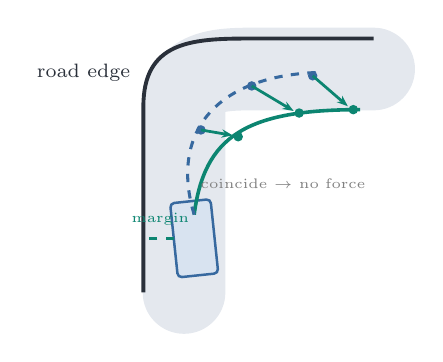
\begin{tikzpicture}[scale=0.86,>={Stealth[length=4pt]},font=\scriptsize]
      \draw[driveC,line width=1.05cm,line cap=round,line join=round]
        (2.6,0.3) -- (2.6,3.0) .. controls (2.6,3.55) and (3.05,3.6) .. (3.6,3.6) -- (5.4,3.6);
      \draw[edgeC,line width=1.4pt]
        (2.0,0.3) -- (2.0,3.05) .. controls (2.0,4.0) and (2.7,4.05) .. (3.55,4.05) -- (5.4,4.05);
      \node[edgeC,anchor=east] at (1.95,3.55) {road edge};
      % current ego, centred with margin
      \carbox{2.75}{1.1}{-84}{policySoft}{policyC}
      \draw[anchorC,dashed,line width=0.9pt] (2.45,1.1) -- (2.0,1.1);
      \node[anchorC,anchor=south,font=\tiny] at (2.25,1.15) {margin};
      % reference (base / expert) future -- teal solid
      \draw[anchorC,line width=1.3pt]
        (2.75,1.45) .. controls (2.9,2.6) and (3.5,3.0) .. (5.2,3.0);
      \fill[anchorC] (3.4,2.6) circle (2pt);
      \fill[anchorC] (4.3,2.95) circle (2pt);
      \fill[anchorC] (5.1,3.0) circle (2pt);
      % predicted future -- policy dashed, drifting wide
      \draw[policyC,dashed,line width=1.1pt]
        (2.75,1.45) .. controls (2.4,2.6) and (3.0,3.5) .. (4.6,3.55);
      \fill[policyC] (2.85,2.7) circle (2pt);
      \fill[policyC] (3.6,3.35) circle (2pt);
      \fill[policyC] (4.5,3.5) circle (2pt);
      % anchor drag arrows
      \draw[anchorC,line width=1pt,->] (2.85,2.7) -- (3.32,2.62);
      \draw[anchorC,line width=1pt,->] (3.6,3.35) -- (4.22,2.98);
      \draw[anchorC,line width=1pt,->] (4.5,3.5) -- (5.02,3.05);
      \node[gray,font=\tiny,anchor=west] at (2.7,1.9) {coincide $\to$ no force};
    \end{tikzpicture}\\[2pt]
    {\scriptsize\textcolor{anchorC}{---}~base/expert line
     ~~\textcolor{policyC}{--\,--}~model prediction}
  \end{columns}
  \vspace{1pt}
  \footnotesize Why base, not the human log? The pretrained policy departs from
  the log \emph{while still succeeding} --- pulling toward the log perturbs a
  working policy. ($\mu_{\text{base}}$ stop-gradiented; rng split fresh per step.)
\end{frame}

% ------------------------------------------------------------------
\begin{frame}{Why $\beta>0$: without the anchor, the successes collapse}
  \small
  \begin{columns}[T]
    \column{0.44\textwidth}
    Run the \emph{identical} safety objective with the anchor off ($\beta{=}0$)
    and it does exactly what the degeneracy predicts: it buys clearance by
    \textbf{wandering off the demonstrated line}.
    \begin{itemize}\itemsep2pt
      \item $\beta{=}0$: success-held-out \bad{$0.98\!\to\!0.59$}, rollout drift
            $0.5\!\to\!6.2$\,m. Bigger raw failure gain, but a \bad{net loss}.
      \item $\beta{=}100$: success-held-out \good{flat at $\sim\!0.98$} while the
            safety term still lands its failure-set gain.
    \end{itemize}
    \begin{alertblock}{The point}
      The safety term has no idea the car is supposed to go somewhere. The
      anchor is not optional.
    \end{alertblock}

    \column{0.56\textwidth}
    \centering
    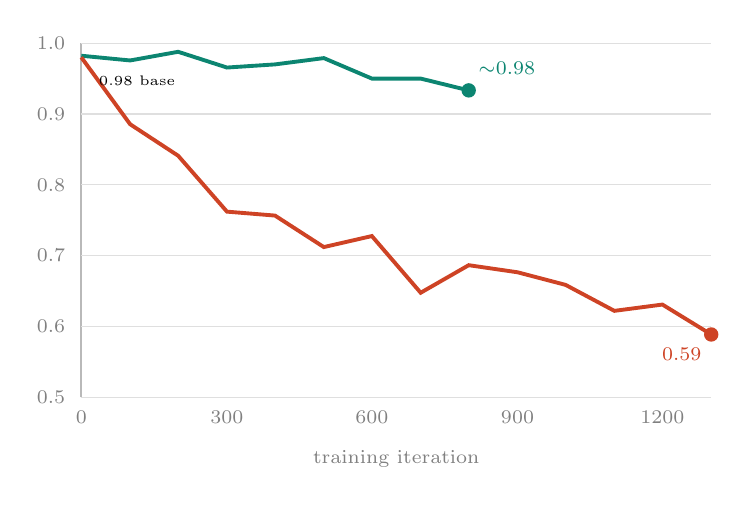
\begin{tikzpicture}[font=\scriptsize]
      % axes frame
      \draw[gray!55,line width=0.8pt] (0,0) -- (0,4.5);
      \foreach \v/\y in {0.5/0,0.6/0.9,0.7/1.8,0.8/2.7,0.9/3.6,1.0/4.5}{
        \draw[gray!25] (0,\y) -- (8,\y);
        \node[gray,anchor=east] at (-0.08,\y) {\v};}
      \foreach \it/\x in {0/0,300/1.85,600/3.69,900/5.54,1200/7.38}{
        \node[gray,anchor=north] at (\x,-0.05) {\it};}
      \node[gray,anchor=north] at (4,-0.55) {training iteration};
      % beta=100 (anchor, teal)
      \draw[anchorC,line width=1.4pt]
        plot coordinates {(0,4.34)(0.62,4.28)(1.23,4.39)(1.85,4.19)(2.46,4.23)
                          (3.08,4.31)(3.69,4.05)(4.31,4.05)(4.92,3.90)};
      % beta=0 (safety only, red)
      \draw[safetyC,line width=1.4pt]
        plot coordinates {(0,4.32)(0.62,3.47)(1.23,3.07)(1.85,2.36)(2.46,2.31)
                          (3.08,1.91)(3.69,2.05)(4.31,1.33)(4.92,1.68)(5.54,1.59)
                          (6.15,1.43)(6.77,1.10)(7.38,1.18)(8.0,0.80)};
      \fill[safetyC] (8.0,0.80) circle (2.6pt);
      \fill[anchorC] (4.92,3.90) circle (2.6pt);
      \node[safetyC,anchor=north east,font=\scriptsize] at (8.0,0.75) {0.59};
      \node[anchorC,anchor=south west,font=\scriptsize] at (4.92,3.98) {$\sim$0.98};
      \node[anchor=west,font=\tiny] at (0.1,4.02) {0.98 base};
    \end{tikzpicture}\\[2pt]
    {\scriptsize held-out \textbf{success} solved-rate ---
     \textcolor{safetyC}{$\beta{=}0$} vs.\ \textcolor{anchorC}{$\beta{=}100$}}
  \end{columns}
\end{frame}


% ##################################################################
\section{Result}
% ##################################################################

% ------------------------------------------------------------------
\begin{frame}{Best marginal run: $\beta=100$, success-anchored}
  \small
  Pick by \textbf{marginal solved-rate} (corpus-weighted blend of failure +
  success splits). \texttt{beta100\_succ} @ iter 200 tops it (0.977), edging
  \texttt{beta100\_all} (0.976) while retaining fractionally more success.
  \begin{center}
  \begin{tabular}{@{}lrrrr@{}}
    \toprule
    held-out split (solved-rate) & base & \textbf{$\beta{=}100$ succ} & $\Delta$ & $\beta{=}0$ only \\
    \midrule
    \textbf{failure set}   & 0.173 & \textbf{0.309} & \good{$+0.136$} & 0.428 \\
    \quad --\,offroad rate & 0.431 & 0.283          & \good{$-0.148$} & 0.269 \\
    \textbf{success set}   & 0.982 & \textbf{0.988} & \good{$+0.006$} & \bad{0.589} \\
    \quad --\,drift (m)    & 0.49  & 0.61           & $+0.12$         & \bad{6.21} \\
    \textbf{marginal}      & 0.970 & \textbf{0.977} & \good{$+0.007$} & \bad{0.586} \\
    \bottomrule
  \end{tabular}
  \end{center}
  \begin{itemize}\itemsep1pt
    \item The failure-set gain (\good{$+0.14$}) comes \emph{with} the safety
          term's job done: offroad $0.43\!\to\!0.28$, success held at $0.99$.
    \item $\beta{=}0$ reaches a higher raw failure number (0.43) only by
          \bad{destroying} the success set ($0.98\!\to\!0.59$, drift
          $0.5\!\to\!6.2$\,m) --- its marginal is a net loss.
  \end{itemize}
  \footnotesize\textcolor{gray}{sweep 20260908\_225908 $\cdot$ verified splits
  $\cdot$ eval seed 12345 $\cdot$ per-run iter-0 baseline (same protocol).}
\end{frame}
